\documentclass[../main]{subfiles}

\questiontrue
\solutiontrue

\begin{document}
    \ifquestion
    
	\section{Miraculous Escape}

You, one of the analysts of the ABFire empire, were studying a curious dust cloud in a strange planetary system. In your studies, you wished to enter the cloud and study it more closely; however, you only realized that there was a black hole inside the cloud. Too late! Your SPS (Space Positioning System) failed, and you lost control of the spacecraft. Only one resource was working: the emergency button. This button, when activated, can send the spacecraft on a parabolic escape trajectory in a desired direction. You, however, do not know which direction to take or how far you are from the black hole. Trying to calm yourself, you decide to find the probability of successfully escaping by choosing a random direction.

Consider that the radius of the black hole's event horizon is $R_b$ and the radius of the cloud is $R_n$.

\ut{a} Find the relation between the angle of the position vector and the velocity vector for the spacecraft to \textbf{enter} the event horizon, for a given position $r$.

\ut{b} Find the probability of the spacecraft escaping from a given position $r$.

\ut{c} Find the probability that the spacecraft is located at a distance $r$.

\ut{d} Determine the probability of the spacecraft escaping, considering that the radius of the black hole is $R_b=69 \cdot 10^6$ m and the radius of the cloud is $R_n=420 \cdot 10^{7}$ m.

Given:

\[
\frac{1}{R_n^3-R_b^3}\int_{R_b}^{R_n}\sqrt{1-\frac{R_b}{r}}\,r^2\,dr \approx 0.2895485
\]

\clearpage

\fi

\ifsolution

\section{Miraculous Escape}

\ut{a} Consider the following diagram:

	\begin{figure}[htpb]
	    \centering
	    

\tikzset{every picture/.style={line width=0.75pt}} %set default line width to 0.75pt        

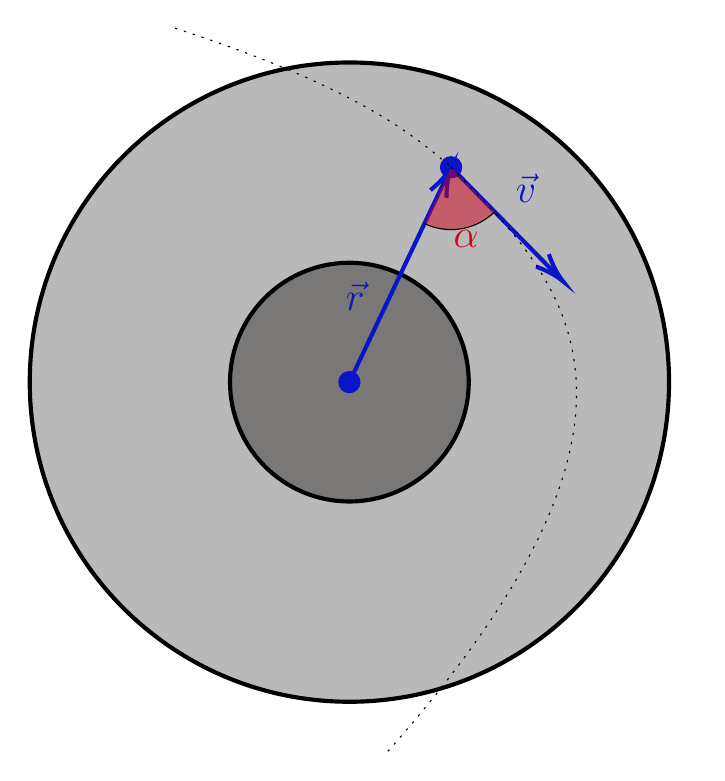
\begin{tikzpicture}[x=0.75pt,y=0.75pt,yscale=-1,xscale=1]
%uncomment if require: \path (0,643); %set diagram left start at 0, and has height of 643

%Shape: Circle [id:dp4615882931559956] 
\draw  [fill={rgb, 255:red, 155; green, 155; blue, 155 }  ,fill opacity=0.7 ][line width=1.5]  (210,322.67) .. controls (210,237.62) and (278.95,168.67) .. (364,168.67) .. controls (449.05,168.67) and (518,237.62) .. (518,322.67) .. controls (518,407.72) and (449.05,476.67) .. (364,476.67) .. controls (278.95,476.67) and (210,407.72) .. (210,322.67) -- cycle ;
%Shape: Circle [id:dp6887912150706346] 
\draw  [fill={rgb, 255:red, 110; green, 106; blue, 106 }  ,fill opacity=0.83 ][line width=1.5]  (306.5,322.67) .. controls (306.5,290.92) and (332.24,265.17) .. (364,265.17) .. controls (395.76,265.17) and (421.5,290.92) .. (421.5,322.67) .. controls (421.5,354.43) and (395.76,380.17) .. (364,380.17) .. controls (332.24,380.17) and (306.5,354.43) .. (306.5,322.67) -- cycle ;
%Straight Lines [id:da5798582116601463] 
\draw [color={rgb, 255:red, 10; green, 20; blue, 200 }  ,draw opacity=1 ][line width=1.5]    (364,322.67) -- (411.72,221.88) ;
\draw [shift={(413,219.17)}, rotate = 115.33] [color={rgb, 255:red, 10; green, 20; blue, 200 }  ,draw opacity=1 ][line width=1.5]    (14.21,-4.28) .. controls (9.04,-1.82) and (4.3,-0.39) .. (0,0) .. controls (4.3,0.39) and (9.04,1.82) .. (14.21,4.28)   ;
\draw [shift={(364,322.67)}, rotate = 295.33] [color={rgb, 255:red, 10; green, 20; blue, 200 }  ,draw opacity=1 ][fill={rgb, 255:red, 10; green, 20; blue, 200 }  ,fill opacity=1 ][line width=1.5]      (0, 0) circle [x radius= 4.36, y radius= 4.36]   ;
%Straight Lines [id:da8103668123600853] 
\draw [color={rgb, 255:red, 10; green, 20; blue, 200 }  ,draw opacity=1 ][line width=1.5]    (413,219.17) -- (464.9,272.03) ;
\draw [shift={(467,274.17)}, rotate = 225.53] [color={rgb, 255:red, 10; green, 20; blue, 200 }  ,draw opacity=1 ][line width=1.5]    (14.21,-4.28) .. controls (9.04,-1.82) and (4.3,-0.39) .. (0,0) .. controls (4.3,0.39) and (9.04,1.82) .. (14.21,4.28)   ;
\draw [shift={(413,219.17)}, rotate = 45.53] [color={rgb, 255:red, 10; green, 20; blue, 200 }  ,draw opacity=1 ][fill={rgb, 255:red, 10; green, 20; blue, 200 }  ,fill opacity=1 ][line width=1.5]      (0, 0) circle [x radius= 4.36, y radius= 4.36]   ;
%Shape: Arc [id:dp3066852578546557] 
\draw  [draw opacity=0][fill={rgb, 255:red, 208; green, 2; blue, 27 }  ,fill opacity=0.5 ] (434,240.6) .. controls (428.59,245.9) and (421.18,249.17) .. (413,249.17) .. controls (408.47,249.17) and (404.17,248.17) .. (400.32,246.37) -- (413,219.17) -- cycle ; \draw   (434,240.6) .. controls (428.59,245.9) and (421.18,249.17) .. (413,249.17) .. controls (408.47,249.17) and (404.17,248.17) .. (400.32,246.37) ;  
%Curve Lines [id:da4075938435087889] 
\draw  [dash pattern={on 0.84pt off 2.51pt}]  (413,219.17) .. controls (465,272.17) and (531,333.17) .. (382,501.17) ;
%Curve Lines [id:da5896793725384881] 
\draw  [dash pattern={on 0.84pt off 2.51pt}]  (280,152.17) .. controls (370,181.17) and (398,206.17) .. (413,219.17) ;

% Text Node
\draw (361,273.07) node [anchor=north west][inner sep=0.75pt]  [font=\Large,color={rgb, 255:red, 10; green, 20; blue, 200 }  ,opacity=1 ]  {$\vec{r}$};
% Text Node
\draw (443,221.07) node [anchor=north west][inner sep=0.75pt]  [font=\Large,color={rgb, 255:red, 10; green, 20; blue, 200 }  ,opacity=1 ]  {$\vec{v}$};
% Text Node
\draw (413,248.07) node [anchor=north west][inner sep=0.75pt]  [font=\Large,color={rgb, 255:red, 208; green, 2; blue, 27 }  ,opacity=1 ]  {$\alpha $};


\end{tikzpicture}
	
\caption{Representation of the spacecraft's parabolic trajectory at a given distance from the black hole's center}
\label{fig:blackholee}
\end{figure}

We will use the law of conservation of angular momentum between the current position and the periapsis:

$$vr\sin{(\alpha)}=v_pr_p$$

Notice that $0 \le \alpha \le \pi$. Knowing that the orbit is parabolic, which implies that the velocity at each point is the escape velocity:

$$\sqrt{\frac{2GM}{r}}\, r \sin{(\alpha)} = \sqrt{\frac{2GM}{r_p}}\, r_p$$

$$\sin{(\alpha)} = \sqrt{\frac{r_p}{r}}$$

Since we want to know the angles for which the periapsis radius is inside the black hole (the spacecraft enters), we set $r_p \le R_b$, which leads to:

$$\sin{(\alpha)} \le \sqrt{\frac{R_b}{r}}$$

\ut{b} By interpreting this result (and observing the unit circle), we find that the angle $\alpha$ is of the form:

$$\alpha \in \left[0, \arcsin{\sqrt{\frac{R_b}{r}}}\right] \cup \left[\pi - \arcsin{\sqrt{\frac{R_b}{r}}}, \pi\right]$$

Illustrating the situation for the spacecraft, we have Figure \ref{fig:doidona}.

\begin{figure}[htpb]
    \centering
    \includegraphics[scale = 0.8]{images/veloci.PNG}
    \caption{Representation of the solid angle and section of the sphere for which escape is possible}
    \label{fig:doidona}
\end{figure}

The spacecraft will have a periapsis inside the black hole if its velocity vector is directed within one of the spherical caps (top or bottom). The total area of the two caps is given by:

$$A_t = 2(A_{\text{cap}}) = 4\pi R^2 (1 - \cos{(\alpha)})$$

Thus, the probability that the velocity lies within one of these areas is the ratio between this area and the total area ($4\pi R^2$):

$$P = 1 - \cos{(\alpha)}$$

To calculate the probability that the spacecraft escapes, we first compute the probability of **not escaping** and then subtract this from 1 to obtain the desired probability.  

One might expect the probability of not escaping to be $P$, but it is possible that the spacecraft is moving in the opposite direction; that is, even if the periapsis is inside the black hole, it could be moving away or toward it (in one case the angle is $\alpha$, in the other it is $\pi - \alpha$). For one of these cases, the spacecraft will still pass through periapsis (and never return), and for the other, it is as if it has already passed. Therefore, the probability of not escaping should be:

$$P_{\text{NS}} = \frac{P}{2} = \frac{1 - \cos{(\alpha)}}{2}$$

Substituting the values and knowing that $(\sin{(\alpha)})^2 + (\cos{(\alpha)})^2 = 1$, we can find the probability of escaping:

$$P_S = \frac{1 + \sqrt{1 - \frac{R_b}{r}}}{2}$$

\ut{c} The probability that the spacecraft is located at a distance $r$ from the black hole is the ratio between the infinitesimal volume element of a sphere of radius $r$ and the total volume of a sphere of radius $R_n$ minus a sphere of radius $R_b$ (since the spacecraft is not inside the black hole):

$$P_r = \frac{d\left(\frac{4}{3}\pi r^3\right)}{\frac{4}{3}\pi (R_n^3 - R_b^3)} = \frac{3 r^2 dr}{R_n^3 - R_b^3}$$

\ut{d} By the multiplicative principle, the probability that the spacecraft is at a distance $r$ and escapes is:

$$dP(r) = P_S P_r$$

Thus, the total probability of escaping is the integral of this function from $R_b$ to $R_n$:

$$P = \int_{R_b}^{R_n} \frac{1 + \sqrt{1 - \frac{R_b}{r}}}{2} \frac{3 r^2 dr}{R_n^3 - R_b^3}$$

$$P = \frac{3}{2(R_n^3 - R_b^3)} \int_{R_b}^{R_n} \left(1 + \sqrt{1 - \frac{R_b}{r}}\right) r^2 dr$$

We can separate the integral into two parts:

$$\int_{R_b}^{R_n} \left(1 + \sqrt{1 - \frac{R_b}{r}}\right) r^2 dr = \int_{R_b}^{R_n} r^2 dr + \int_{R_b}^{R_n} \sqrt{1 - \frac{R_b}{r}} r^2 dr$$

The first integral is trivial:

$$\int_{R_b}^{R_n} r^2 dr = \frac{R_n^3 - R_b^3}{3}$$

The second integral can use the provided value from the problem statement, giving:

$$P = \frac{3}{2(R_n^3 - R_b^3)} \left( \frac{R_n^3 - R_b^3}{3} + 0.2895485 (R_n^3 - R_b^3) \right)$$

Finally, we find that:

	$$P=93.43 \%$$
	
	\clearpage
    
    
    \fi
\end{document}
